\chapter{Background}
\label{chap:background}


\section{Mining Open Source Software Repositories}

% TODO ensure this is accurate.
\gls{oss} generally is software that provides with the ability access the source code and make modifications to the source code. While certain licenses provide some restrictions on the ability to redistribute the software the main point of the source code of the software being freely available is key. The scope and capability of \gls{oss} projects vary greatly. Several very popular \gls{oss} projects are listed in table \ref{tab:oss_projects}.

%TODO make sure footnotes fit in better.
\begin{table}[h!]
\begin{minipage}{\textwidth}
\begin{center}
    \begin{tabular}{|l|l|l|}
        \hline
        Owner & Project & Description \\
        \hline

        Mozilla & Firefox\footnote{\url{https://www.mozilla.org/en-US/firefox/desktop/}} & Internet Browser \\
        Linux & Linux Kernel\footnote{\url{https://www.kernel.org/}} & Operation System Kernel \\
        VideoLAN & VLC\footnote{\url{http://www.videolan.org/vlc/index.html}} & Media Player \\
        PostgreSQL & PostgreSQL\footnote{\url{http://www.postgresql.org/}} & Object-Relational Database Management System \\
        git & git\footnote{\url{https://git-scm.com/}} & Version Control System \\
        \hline
    \end{tabular}
\end{center}
\caption{Open Source Software Projects}
\label{tab:oss_projects}
\end{minipage}
\end{table}
%Firefox => MPL 2.0
%Linux Kernel => GPL v2, plus various closed-source binary blobs
%VLC => GPLv2+ (player), LGPLv2.1+ (engine)
%PostgreSQL => PostgreSQL License
%git => GNU General Public License v2, GNU Lesser General Public License 2.1

The development of large software projects (whether \gls{oss} or not) often make use of \gls{vcs}. A \gls{vcs} helps the developers of the project manage the changes of the project and facilitate the collaboration between developers. A \gls{vcs} will keep an current version of the project and keep track of the previous version of the project as well. This may be done through keeping a copy of each version of the project or by keeping track of all each change made to the project. \gls{svn} and git would be two examples of \gls{vcs}s.

Git is a \gls{dvcs} and differs greatly from \gls{svn} which is a normal \gls{vcs}. Git will provide the user with a complete copy of the repository that is worked on independent of network connection. The independence of each repository also allows for a repository to be developed without a centralized server. The distributed aspect of git tends to allows for easier use for all involved parities. The one main issue with a \gls{dvcs} is that while decentralization is useful, developers will require some method to collaborate and communicate to transfer changes made to the repository. Therefore typically one centralized server is used to maintain communication between all interested parties.

Git has grown in popularity since it was created and is at the core of several \gls{vcm} sites such as GitHub \footnote{\url{https://github.com/}}, BitBucket \footnote{\url{https://bitbucket.org/}} and GitLab \footnote{\url{https://gitlab.com/}}. These platforms tend to be fairly supportive of \gls{oss} projects through providing their services free of charge. For example, GitHub provides unlimited public repositories completely free. While these projects do not have to be licensed with an open source license typically they will be since they are already publicly visible.

% GitLab -> https://gitlab.com/
% GitHub -> https://github.com/
% BitBucket -> https://bitbucket.org/

GitHub is the most popular of the \gls{vcm} websites and hosts numerous very popular \gls{oss} projects including, the Linus Kernel, Swift\footnote{\url{https://swift.org/}} and React\footnote{\url{https://facebook.github.io/react/}}. GitHub also provides a public \gls{api} to allow for access to the data related to project repositories which is discussed further below. % TODO link to that.
Given the popularity of GitHub for use by developers and the availability of the project data, GitHub is an obvious choice for mining project data. Especially since the goal of mining software is to capture \gls{oss} project data to both explore and test analysis methods. Publicly visible projects are also publicly accessible through the \gls{api} and the majority are open source.

%%%%%%%%%%

Git provides a simple interface to manage the repository regardless of which site is the central server. Therefore regardless which site the project resides on users can easily interact with the project as long as they know the git interface. Git in essences is a file storage for the project that keeps track of changes made to the project. A \textit{commit} is a set of changes that a developer has made at a certain time. The developer has full control what gets committed, when it gets committed and even modified at a later date.
%This results in the date of the commit merely identifying when the developer formally notified Git that a change was made.

A branch is a series of commits that are often related. In figure \ref{fig:network_diagram}, each dot would represent a commit and a set of dots connected by the same colored lines are a branch. Branches can be considered different paths or deviations in the development from each other allowing for different versions of the project to be maintained and developed. The \textit{master} branch is the main branch, represented with black, from which all branches usually stem from and is generally where projects are developed on. On a similar note, a \textit{tag} is a branch that is frozen to allow for future reference. Tags are often uses to mark a significant point in the development history such as a project release. Finally, when two differently branches converge into a single dot then the two branches have been \textit{merged}. A merge indicates that the differences between the two branches are consolidated based on the developer's discretion.

\begin{figure}[!ht]
    \centering
        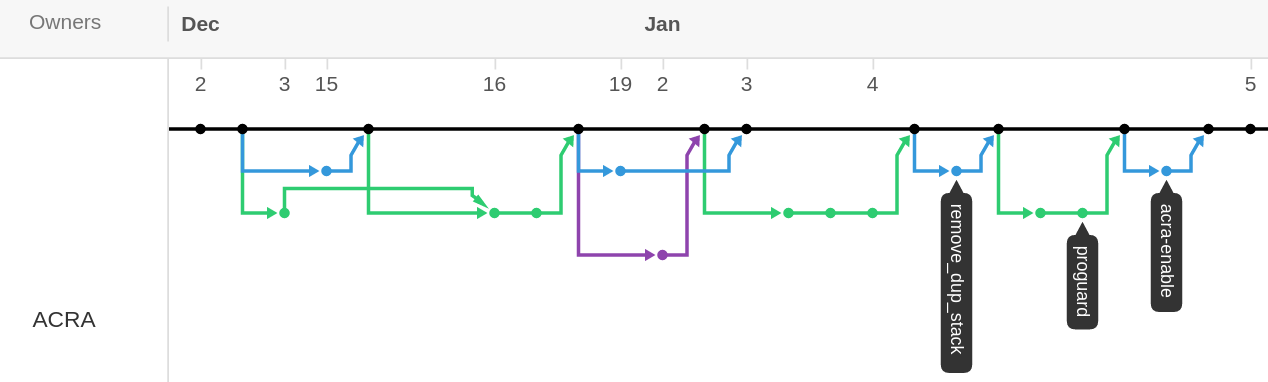
\includegraphics[width=1.0\textwidth]{images/network}
    \caption{Network diagrams}
    \label{fig:network_diagram}
\end{figure}

A commit consists of files that have been changed, more specifically a list of \textit{patch} files which each outline the changes made to their corresponding file. The patch file consists of a series of differences between the previous version of the file and this new version of the file. These patch files are key since they contain the actual changes made to the project and thus are the major point of interest.

% TODO fix close

\section{Machine Learning}

% Rase, realizing software engineering learning
Machine learning is a complex method for software algorithms to attempt to determine patterns within the data. One such problem example would be an algorithm to detect certain people within an image. For an individual such a task may seem trivial however for a software system to detect it is far more difficult. Algorithms that can determine patterns and mimic them from abstract set of data is useful when such patterns are extremely complex. A few examples of such algorithms are \gls{svm}, ...


\section{Change Prediction}

% Related work stuff here or later

The development of large scale projects can take a long time and involve a huge time investment from the developers. The development of the project will cause for the developers to make changes to projects. Software projects will have faults within the project especially during the development phase. A project in its early stages may not meet the full set of functionality since it has not been completed yet. Since the development team will known that such features are not yet implemented these faults or fails are not a huge concern. Rather faults that are unknown to the developer team are far more serious. Such cases as a feature was thought to be implemented correct but was not or a feature implementation breaks other features. In both those cases changes made to the project cause the fault to be revealed.

Changes to the project are the means by which all development occurs. The ability to analyze and predict changes within a project could give deep insights into the development of a project. 

% TODO talk about previous work on change prediction. cause. 